\documentclass[a4paper]{IEEEtran}
\pagestyle{empty}

\usepackage{booktabs}
\usepackage{graphicx}
\usepackage{url}
\usepackage[top=2.4cm,left=1.5cm,right=1.5cm,bottom=3.5cm]{geometry}
\usepackage{listings}
\usepackage{amssymb}
\usepackage{siunitx}
\usepackage{circuitikz}
\usepackage[style=ieee]{biblatex}

\addbibresource{ref.bib}
\graphicspath{{figures/}}
\setlength{\columnsep}{0.24in}
\setlength{\headsep}{0in}
\setlength{\parindent}{1.2pc}

\begin{document}

\title{Electromagnetic Characterisation of a Short-Stroke Ferromagnetic Actuator}
\author{R. M. Inston and H. Karimjee}

\maketitle
% \begin{abstract}
% This experiment demonstrated the use of FEMM as an analysis tool for a short stroke ferromagnetic actuator. 
% \end{abstract}

\section{Nomenclature}
    \begin{itemize}
    \item[]{$R_{w}$, Winding resistance, [$\Omega$]}
    \item[]{$l_{w}$, Length into the page of winding, [m]}
    \item[]{$A_{w}$, Area of winding, [m$^{2}$]}
    \item[]{$V_{w}$, Volume of winding, [m$^{3}$]}
    \item[]{$N$, Number of turns in the winding, [-]}
    \item[]{$\sigma$, Conductivity of winding, [Sm$^{-1}$]}
    \item[]{$k_{PF}$, Packing factor of conductors in the winding, [-]}
    \item[]{$L$, Inductance of the winding, [H]}
    \item[]{$\mathcal{R}$, Reluctance, [H$^{-1}$]}
    \item[]{$A_{eff}$, Effective area of air gap, [m$^{2}$]}
    \item[]{$W$, Width of air gap, [m]}
    \item[]{$T$, Thickness of air gap, [m]}
    \item[]{$g$, Air gap length, [m]}
    \end{itemize}

\section{Introduction}
% COULD PROBABLY DO WITH BULKING UP A BIT

    Finite Element Method Magnetics (FEMM) is an implementation of Finite Element Analysis (FEA) that specialises in electro-magnetics. This tool, in combination with MATLAB or another scripting language such as Python, can be used to create a series of numerical simulations, from which a electro-magnetic and then mechanical analysis can be extracted. 
    
    Here, FEMM is being used to characterise a magnetic actuator, outlined in \cite{labPartA}, made up of an armature and a core which share the same ferromagnetic properties, two sets of windings around the top and bottom of the core and three air gaps of note, as in Fig \ref{xsection}. This characterisation will be done in four situations: analytically, neglecting and accounting for fringing, and numerically, using both a linear and non-linear ferromagnetic material. 

    \begin{figure}[ht]
        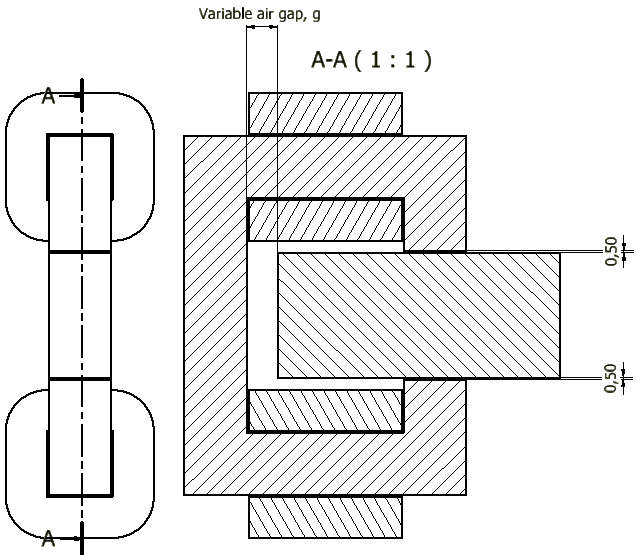
\includegraphics[width = \linewidth]{actuator-2.jpg}
        \caption{Cross-sectional view of the actuator with the three air gaps higlighted (All measurements in mm).}
        \label{xsection} 
    \end{figure}

\section{Model Meshing}

    To perform FEA, a model is split into elements. The elements must be small enough to output an accurate enough answer despite the linearisation of the physics involved, whilst not being too small so as to increase the computational time to an unreasonable length.

    FEMM has a smart-meshing tool in which the software analyses the model and allocates a dense mesh where higher resolution analysis is required and a sparse mesh where it is not. This is evident in the difference between figures \ref{noSmartMesh} \& \ref{smartMesh}. Although useful, this feature increases the mesh elements (see table \ref{meshTable}) without knowing any information about the overarching aim of the problem. This is illustrated at the boundaries of the variable air gap between the movable armature and core, which is vital for the analysis of the force-displacement characteristic of the actuator. Smart-meshing fails to recognise these edges as paramount to the analysis and produces a grid seen in Fig \ref{zoomNotDense}. By manually setting the spacing of meshing along these lines as suggested in \cite{labPartB} Section II, FEMM can produce a denser, more regular mesh as seen in Fig \ref{zoomDense}. This accuracy has its cost in terms of mesh elements (Table \ref{meshTable}) and computational time; in running larger simulations than the ones carried out here, careful thought should be put into which areas of a model require more accurate analysis to avoid excessive computational requirements but maintaining a valid output.

    \begin{figure}[ht]
        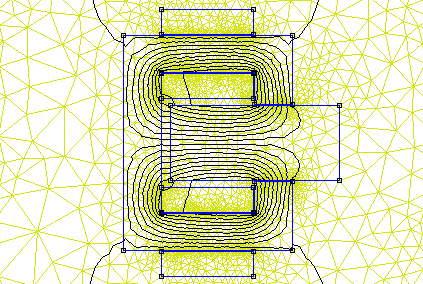
\includegraphics[width = \linewidth]{Smartmesh-OFF-NotDenseAirgap.png}
        \caption{Example mesh with smart-meshing disabled. Note the sparseness of the triangulation.}
        \label{noSmartMesh} 
    \end{figure}

    \begin{figure}[ht]
        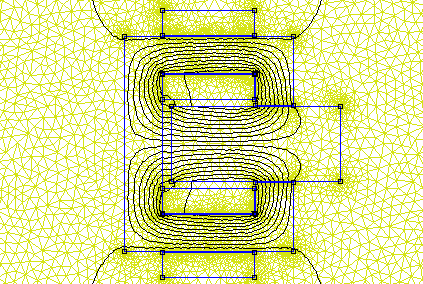
\includegraphics[width = \linewidth]{Smartmesh-ON-NotDenseAirgap.png}
        \caption{Example mesh with smart meshing enabled. Note how the density increases around boundaries of interest.}
        \label{smartMesh} 
    \end{figure}

    \begin{figure}[ht]
        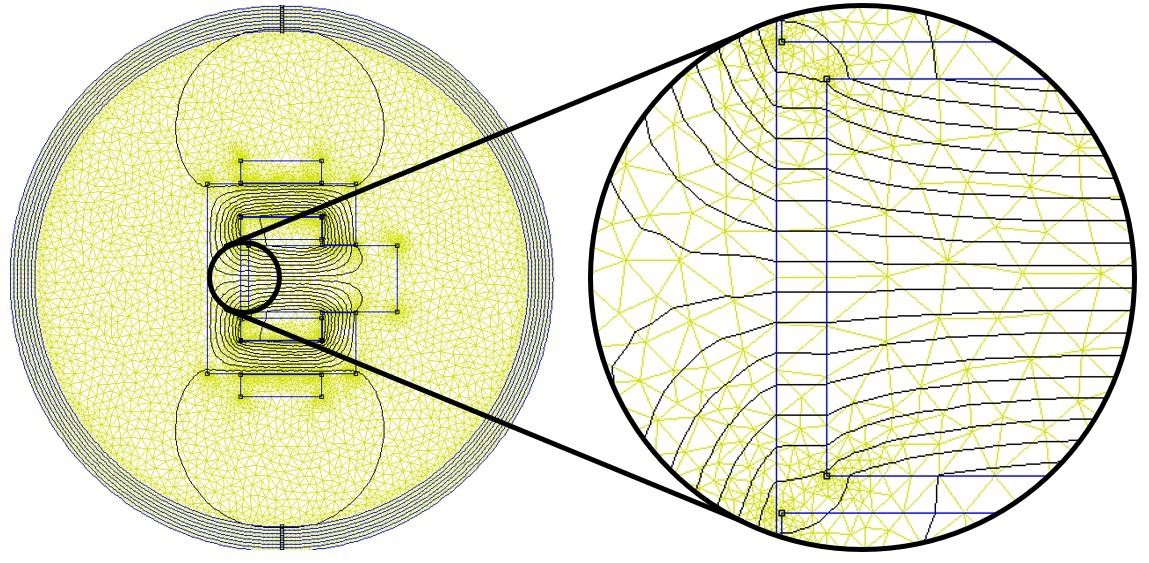
\includegraphics[width = \linewidth]{figurezoomnotdense.jpg}
        \caption{FEMM smart-meshing output without specifying the area of interest. The density is low despite smart-meshing being on.}
        \label{zoomNotDense} 
    \end{figure}

    \begin{figure}[ht]
        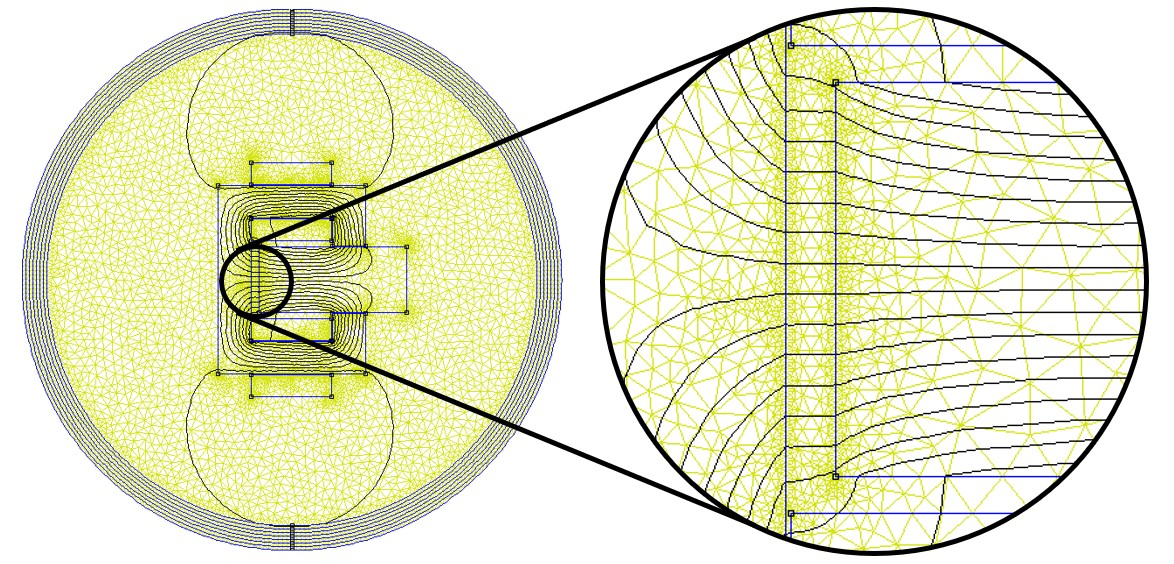
\includegraphics[width = \linewidth]{figurezoomdense.jpg}
        \caption{FEMM smart-meshing output with specifying the area of interest and increasing the density of mesh elements within.}
        \label{zoomDense} 
    \end{figure}

    \begin{table}[ht]
        \centering
            \begin{tabular}{ccc}
            \textbf{\begin{tabular}[c]{@{}c@{}}Smart-\\ meshing\end{tabular}} & \textbf{\begin{tabular}[c]{@{}c@{}}Dense\\ Air gap\end{tabular}} & \textbf{\begin{tabular}[c]{@{}c@{}}Mesh\\ Elements\end{tabular}} \\ \hline
            \multicolumn{1}{l}{} & \multicolumn{1}{l}{} & \multicolumn{1}{l}{} \\
            OFF & OFF & 14790 \\
            OFF & ON & 16334 \\
            ON & OFF & 22668 \\
            ON & ON & 24368 \\
            \multicolumn{1}{l}{} & \multicolumn{1}{l}{} & \multicolumn{1}{l}{}
            \end{tabular}
        \caption{A summary of meshing options for the model.}
        \label{meshTable}
    \end{table}


\section{Winding Resistance}
    To calculate the winding resistance, $R_{w}$, two approaches were used: extracting resistance from FEMM and analytical. FEMM can calculate the winding resistance by obtaining the voltage and current across and through the winding respectively, and finding the resistance using Ohm's law. The analytical approach used block integrals in FEMM to obtain winding area and volume, and hence the winding depth (into the page) can be found using Eq \ref{length}:

    \begin{equation}
        l_{w} = \frac{V_{w}}{A_{w}}
        \label{length}
    \end{equation}

    The analytical resistance is thus calculated using Eq \ref{resistance}. The resistances of each calculation method are presented in table \ref{windingResistance}. 

    \begin{equation}
        R_{w} = \frac{N l_{w}}{\sigma\left(\frac{k_{PF} A_{w}}{N}\right)}
        \label{resistance}
    \end{equation}

    Table \ref{windingResistance} shows a significant difference in estimated values. The analytical value uses a packing factor, \(k_{PF} = 0.6\), that compensates for the space used by the insulating material in a winding. FEMM sees the entire area as conducting material and hence the implied cross sectional area of wire increases. Given the conductivity \(\sigma = 58 \si{MS/m}\) in both predictions, the greater the implied length of winding, the greater the winding resistance, $R_{w}$. However, FEMM is working with a 2D model and the analysis was performed on the top and bottom sections of the winding only. This means the analysis does not account for the whole length around the winding, notably the rounded corners and sides, causing the FEMM estimate to be at least a factor of four smaller than the analytical prediction. 
    
    
    \begin{table}[ht]
        \centering
            \begin{tabular}{c|cc}
            \textbf{Method} & \textbf{Current {[}A{]}} & \textbf{\begin{tabular}[c]{@{}c@{}}Winding\\ Resistance {[}$\Omega${]}\end{tabular}} \\ \hline
            &  &  \\
            FEMM & 10 & 0.0107 \\
            Analytical & 10 & 0.0557
            \end{tabular}
        \caption{A summary of winding resistance calculation for different methods.}
        \label{windingResistance}
    \end{table}

    The resistances resulting from these two methods were used to calculate the power loss through the windings for a range of current values using Eq \ref{powerLoss}. This was then plotted giving the graph in Fig \ref{windingLoss}. Clearly, this shows the power loss based on the analytically calculated resistance quickly becomes far greater than that of the FEMM calculated resistance. As such, if the analysis performed on the actuator were to be taken further into real applications, the analytical power loss should be considered when specifying power dissipation requirements, rather than the FEMM output. 

    \begin{equation}
        P_{loss} = I^2 R
        \label{powerLoss}
    \end{equation}
    
    \begin{figure}[ht]
        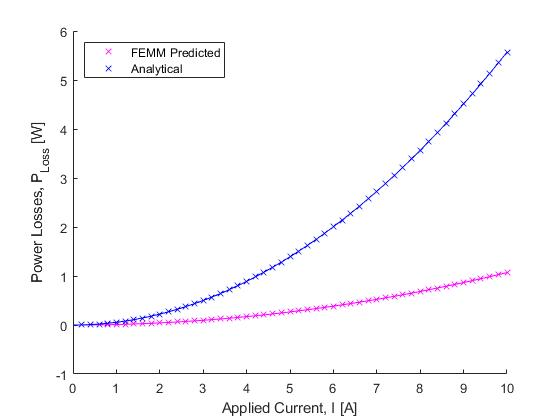
\includegraphics[width = \linewidth]{ResistanceWindingLoss.jpg}
        \caption{Power loss against current based on Eq \ref{powerLoss} for analytical and FEMM calculated resistances. A quadratic curve produces the line of best fit.}
        \label{windingLoss} 
    \end{figure}

\label{windRes}

\section{Winding Inductance}
    Similarly to the winding resistance, the inductance of the windings can be found analytically and numerically. The value can be calculated analytically with Eq \ref{inductance}. 

    \begin{equation}
        L = \frac{N^2}{\sum{\mathcal{R}}}
        \label{inductance}
    \end{equation}

    Assuming flux is conserved, the total reluctance can be calculated based on a magnetic equivalent circuit, Fig \ref{magCircuit}. Note this is only half of the complete circuit for the actuator.


    \begin{equation}
        \sum{\mathcal{R}} = \mathcal{R}_{core} + \mathcal{R}_{air} + \mathcal{R}_{armature} + \mathcal{R}_{gap}
        \label{summm}
    \end{equation}

    \begin{equation}
        \mathcal{R} =  \frac{l}{\mu_{0}\mu_{r}A}
        \label{reluctance}
    \end{equation}
    

    To improve accuracy, fringing effects can be taken into account by replacing $A$ in  Eq \ref{reluctance} with $A_{eff}$ from Eq \ref{EffectiveArea} for $\mathcal{R}_{airgap}$ and $\mathcal{R}_{variable}$. 

    \begin{equation}
        A_{eff} = (W + 2g)(T + 2g)
        \label{EffectiveArea}
    \end{equation}

    \begin{figure}[ht]
        \centering
        \begin{circuitikz}[scale=0.65, european]
            \draw
            (0,0) to[american voltage source=$NI_{winding1}$, invert] (0,3)
            to[R=$\mathcal{R}_{core}$] (3,3) to[R=$\mathcal{R}_{air gap}$] (6,3)
            to[vR=$\mathcal{R}_{armature}$] (6,0)
            to[vR=$\mathcal{R}_{variable}$] (0,0);
        \end{circuitikz}
        
        \caption{Half equivalent magnetic circuit for the ferromagnetic actuator.}
        \label{magCircuit}
    \end{figure}

    As only half of the equivalent circuit (shown in Fig \ref{magCircuit}) was used to calculate the inductance, the result was doubled to obtain the effective inductance of the whole actuator. To allow for this, only half of the armature and variable air gap areas were used in the original calculation. 

    Assuming flux is conserved and then accounting for fringing gives two analytical values. Numerically, two values of inductance can be obtained from FEMM by using a linear and non-linear approximation of core and armature properties. FEMM outputs winding current and flux linkage for each assigned internal circuit; from this inductance can be calculated with Eq \ref{fluxInductance}. Winding current and flux linkage were obtained for one of the winding circuits, and an inductance calculated. As with the analytical inductance, this was then doubled to obtain the effective total inductance for both windings - only possible as the actuator is symmetrical. 

    \begin{equation}
        L = \frac{\psi}{I}
        \label{fluxInductance}
    \end{equation}

    The variation in inductance with armature displacement is shown in Fig \ref{inductanceGraph}. Clearly, the closer the armature is to the core the greater the inductance. This is the expected behaviour, as from Eq \ref{inductance} a smaller total reluctance will give a larger inductance. The total reluctance is very sensitive to the width of the variable airgap and therefore the armature position. As air has a much smaller relative permeability (\(\mu_r\)) than the core material, a large airgap will dominate the circuit and give a large total reluctance which significantly limits the flux travelling around the circuit, giving a small inductance. As the airgap gets smaller, its reluctance drops and the core material begins to dominate the circuit with its higher relative permeability, leading to a lower total reluctance allowing more flux to travel arond the circuit, giving a higher inductance. The inductance for the non-linear core material shows the effect of saturation: as the armature approaches the closed position (-4.9mm displacement) the inductance doesn't follow the same trend as the numerically simulated linear material and analytical approaches.

    The analytical model accounting for fringing effects has higher inductance at all actuator positions than the model assuming flux is conserved. This is due to fringing increasing the effective area of the airgap and therefore decreasing its reluctance. 
    
    For armature positions close to the core, the analytically calculated (with fringing) and numerically simulated inductances are very similar, which suggests the approximation of fringing effects using Eq \ref{EffectiveArea} is relatively accurate for small airgap sizes. As the airgap increases however, the two inductances diverge significantly, suggesting the approximation is only accurate for small values of g.

    
    \begin{figure}[htb]
        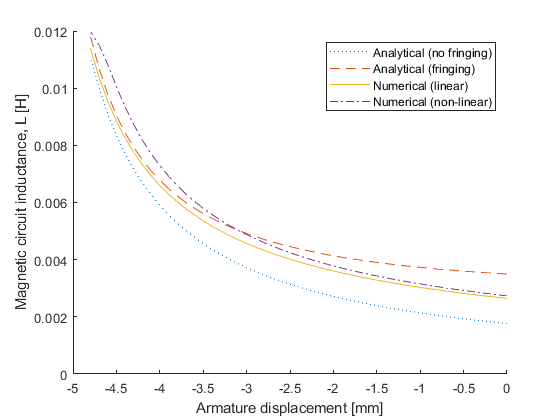
\includegraphics[width = \linewidth]{Inductances.png}
        \caption{Graph showing inductance versus armature displacement for the varying methods of calculation. Armature in open positon has zero displacement.}
        \label{inductanceGraph} 
    \end{figure}


\section{Force on the Armature}
% NEEDS A CHEEKY WRITE UP
% THAT IT DOES

    The method for calculating the force on the armature is outlined in \cite{labPartB} Section VI. In following this method, \(\Psi-I\) diagrams were plotted with \(\Psi\) extracted from FEMM. The change in co-energy between armature positions was found by numerically integrating the area between curves (successive armature positions) in Fig \ref{psi-eye}. The force on the armature between each position was then calculated as in Eq \ref{armatureForce}, effectively taking work done and dividing it by displacement. This was done for 50 armature positions to maximise resolution without excessive computational time.

    The \(\Psi - I\) diagrams for the analytical and numerical linear situations follow the same pattern: \(\Psi\) linearly increasing with \(I\), with a steeper gradient the closer the armature is to the core. This is sensible as the flux able to be pushed around the circuit by the magneto-motive force set up by the windings will increase both as the MMF is increased and as the reluctance of the magnetic circuit decreases. The numerical non-linear case is the most interesting, showing evidence of saturation when the actuator approaches the closed position where the curve begins to tail off. The analytical case with no fringing has the least flux linkage across armature positions as it has the highest reluctance flux path; the one accounting for fringing the highest flux linkage having the lowest reluctance flux path due to the increased airgap area.  

    

    \begin{equation}
        F = \frac{\Delta E_{mech}}{\Delta x}
        \label{armatureForce}
    \end{equation}

    The four force-displacement graphs shown in Fig \ref{forceGraph} have broadly similar characteristics, following an exponential trend where force increases as the armature approaches the closed position. The analytical cases show a higher force in closed position, and lower force in the open position than the linear numerical case, further suggesting that the fringing approximation is imperfect. The non-linear numerical case has the highest force through all armature positions until saturation begins to have an effect, which compared to the linear numerical case suggests the model is non-linear across the whole B-H curve rather than just accounting for saturation. 

    From Fig \ref{forceFEMM} and Table \ref{coenergy}, the force and co-energy calculated using the plotted \(\Psi-I\) curves and those taken from FEMM are almost identical, with values only slightly different at a few displacements. This could be down to small errors in the numerical integration performed on the \(\Psi-I\) curves. That these two curves match also suggests the analysis performed on the data extracted from FEMM in the other cases is also correct, as it followed the same methodology as for the non-linear case here.


    \begin{figure}[ht]
        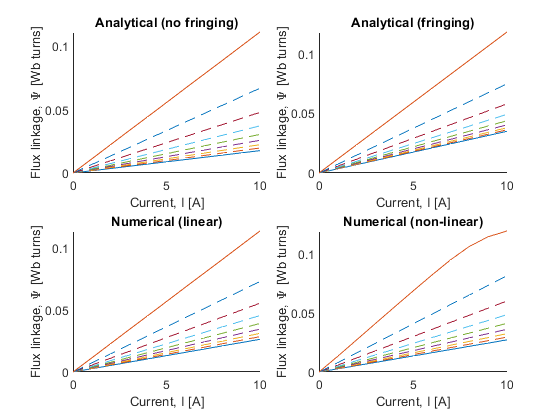
\includegraphics[width = \linewidth]{psi-I-diagrams.png}
        \caption{$\Psi$-I diagrams for the four methods of calculating inductance. Note saturation reached in the non-linear graph. Shown for zero displacement, maximum displacement ($-49$mm) and seven linearly spaced intervals between (dashed lines).}
        \label{psi-eye} 
    \end{figure}

    \begin{figure}[ht]
        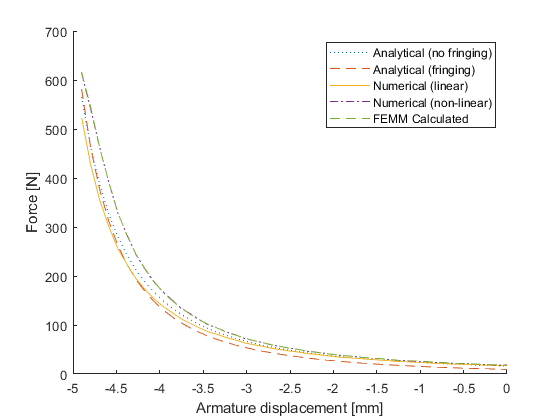
\includegraphics[width = \linewidth]{F-x.png}
        \caption{Force versus displacement for the four methods of calculating inductance. Armature in open position at 0mm.}
        \label{forceGraph} 
    \end{figure}

    \begin{figure}[ht]
        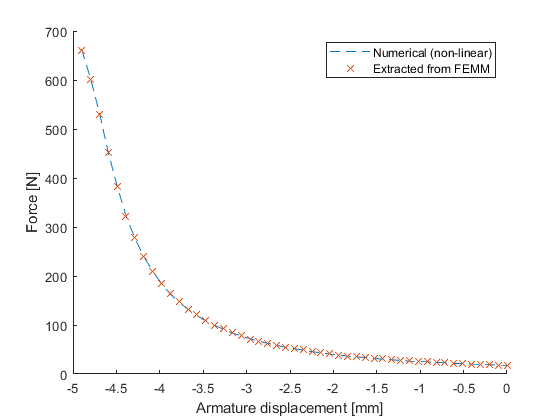
\includegraphics[width = \linewidth]{F-x-FEMM.png}
        \caption{Force versus displacement for the numerical non-linear case and extracted directly from FEMM.}
        \label{forceFEMM} 
    \end{figure}

    \begin{table}[ht]
        \centering
        \begin{tabular}{@{}ccc@{}}
            \toprule
            Displacement {[}mm{]} & $\Delta E_{c_{(\Psi-I)}}$  & $\Delta E_{c_{FEMM}}$   \\ \midrule
            -0.1                  & 0.0018 & 0.0018 \\
            -0.2                  & 0.0018 & 0.0018 \\
            -0.3                  & 0.0019 & 0.0019 \\
            -0.4                  & 0.0020 & 0.0020 \\
            -0.5                  & 0.0020 & 0.0020 \\
            -0.6                  & 0.0021 & 0.0021 \\
            -0.7                  & 0.0022 & 0.0022 \\
            -0.8                  & 0.0023 & 0.0022 \\
            -0.9                  & 0.0023 & 0.0024 \\
            -1.0                  & 0.0025 & 0.0025 \\
            -1.1                  & 0.0026 & 0.0026 \\
            -1.2                  & 0.0026 & 0.0026 \\
            -1.3                  & 0.0027 & 0.0028 \\
            -1.4                  & 0.0029 & 0.0028 \\
            -1.5                  & 0.0031 & 0.0031 \\
            -1.6                  & 0.0032 & 0.0032 \\
            -1.7                  & 0.0033 & 0.0033 \\
            -1.8                  & 0.0035 & 0.0035 \\
            -1.9                  & 0.0037 & 0.0037 \\
            -2.0                  & 0.0038 & 0.0039 \\
            -2.1                  & 0.0041 & 0.0040 \\
            -2.2                  & 0.0044 & 0.0044 \\
            -2.3                  & 0.0045 & 0.0045 \\
            -2.4                  & 0.0049 & 0.0049 \\
            -2.5                  & 0.0052 & 0.0051 \\
            -2.6                  & 0.0055 & 0.0055 \\
            -2.7                  & 0.0058 & 0.0059 \\
            -2.8                  & 0.0062 & 0.0062 \\
            -2.9                  & 0.0067 & 0.0067 \\
            -3.0                  & 0.0071 & 0.0072 \\
            -3.1                  & 0.0079 & 0.0078 \\
            -3.2                  & 0.0084 & 0.0083 \\
            -3.3                  & 0.0092 & 0.0092 \\
            -3.4                  & 0.0098 & 0.0099 \\
            -3.5                  & 0.0108 & 0.0109 \\
            -3.6                  & 0.0121 & 0.0119 \\
            -3.7                  & 0.0131 & 0.0132 \\
            -3.8                  & 0.0148 & 0.0147 \\
            -3.9                  & 0.0164 & 0.0163 \\
            -4.0                  & 0.0183 & 0.0185 \\
            -4.1                  & 0.0210 & 0.0210 \\
            -4.2                  & 0.0239 & 0.0240 \\
            -4.3                  & 0.0279 & 0.0277 \\
            -4.4                  & 0.0322 & 0.0323 \\
            -4.5                  & 0.0383 & 0.0383 \\
            -4.6                  & 0.0452 & 0.0453 \\
            -4.7                  & 0.0529 & 0.0533 \\
            -4.8                  & 0.0601 & 0.0602 \\
            -4.9                  & 0.0659 & 0.0663 \\ \bottomrule   
        \end{tabular}
        \caption{Tabulated data for the change in co-energy between each simulated position. Change given between specified and previous displacements.}
        \label{coenergy}
    \end{table}


\section{Conclusion}
Electro-mechanical systems that use magnetism as the energy transfer medium are difficult to analyse accurately with analytical methods. This is evident from the mathematics that described the force calculation in the analytical cases. As such a numerical tool such as FEMM is preferable, especially when the geometry of the problem is more complex than the actuator in Fig. \ref{xsection}. The different methods of calculation proved to show broadly similar trends except for the extreme armature displacements: saturation became a prominent force when closed and fringing approximations became inaccurate when open. The time taken to perform this analysis was greatly reduced with a linear approximation: the non-linear method embedded in FEMM uses an iterative Newton-Raphson method which is computationally intensive. The context of the problem is therefore important to consider when using this or similar tools: settling for lower accuracy but faster calculation in certain situations might be a sensible choice, however a strong understanding of the underlying concepts is required to confidently make this decision.

There are, however, flaws in this method of characterising the actuator. As discussed in Section \ref{windRes}, the winding resistance calculated in FEMM does not account for end windings due to the 2D planar problem definition. This definition leads to a further limitation: the model cannot account for flux going 'into' or coming 'out of' the page which will have a significant impact on the airgap flux path. As the analysis is performed in a series of magneto-static cases, the model also cannot account for eddy currents induced through the relative motion of the core and armature.

Reluctance actuators such as the one modelled would generally be implemented with a retaining and mechanical returning mechanism for the armature. The actuator can then be used to generate high force vibrations, or in low friction compressors \cite{menerouddesign} for use in hydrogen propellant management in aerospace applications.

\printbibliography

% \pagebreak
% \onecolumn
% \section{Appendix}
% \textsc{\textbf{The following is a listing of the Matlab script written to construct the actuator:}}
% \lstinputlisting[language=Matlab]{construct_actuator_copy.m}

% \pagebreak
% \textsc{\textbf{The following is a listing of the Matlab script written to analyse the actuator:}}
% \lstinputlisting[language=Matlab]{analyse_actuator_copy.m}
 
% \pagebreak
% \textsc{\textbf{The following is a listing of the Matlab script written to produce the graphs and tables:}}
% \lstinputlisting[language=Matlab]{process_copy.m}

\end{document}